\chapter{Background} \label{chap:background}
In order to conduct the comparison effectively, it is necessary to first lay a good theoretical basis of event-driven architecture, event stream processing and the concrete roles of an \acrlong{esp} platform. Based on that, a comprehensive set of evaluation metrics can be determined.
\section{Event Driven Architecture}
In distributed systems comprised of multiple services, these services need to have a mechanism to coordinate and work together to achieve end results. There are typically two approaches for this task, namely, request-driven and event-driven \cite{stopford2018designingeventdriven}. In the first approach, a service sends command to request for state change or queries current state in other services. One advantage of this way is that the state of each service is consistent for all other services since it only exists in one place. However, this method is hard to scale because the control logic concentrates on the sender of requests.

For the latter approach, whenever a service updates its state, it sends out an event. Any other service can listen and operate on this event without the sender knowing about it. This leads to inversion of control where the receiver of events now dictates the operational logic. As a result, services of the system can be more loosely coupled. The events can be used to simply notify receiver about a state change to trigger its reaction usually involving querying for more information from a remote source. One more usage of events is for state replication across the system. Current state of any service can be reconstructed anywhere by applying its published events on the same initial state in the right order. Martin Fowler wrote about two different patterns which are Event-Carried State Transfer and Event-Sourcing \cite{martinfowlereventdriven} but they basically refer to the same way to use event. When a service keeps a state copy of another locally, it can access this data faster and becomes independent of the online status of the source of data. Nevertheless, having multiple copies of data across the system also means that the system can be in inconsistent state temporarily or even worse permanently if it is not designed carefully. Therefore, care should be taken when applying event-driven architecture to not overcomplicate the system.

\section{Event Stream Processing} \label{section:eventstreamprocessing}
With the increasing amount of data, the demand about how data is processed and analyzed also evolves over time. In the early day, data is usually collected over a period of time and stored in a big bounded batch in a data warehouse. Some scheduled batch jobs will then go over the entire batch of data to generate insights and reports tying to the needs of the organization. However, this type of data processing gradually cannot keep up with the need of faster analysis allowing companies to response more timely to change. Therefore, the concept of stream processing begins to emerge.


Unlike its batch counterpart, stream processing aims at handling unbounded data which is a better form for representing the flow of events in real world given their continuous and boundless nature. By processing this influx of data continuously as they arrives, events and patterns can be detected with low latency making stream processing more suitable for real-time use cases. Moreover, the input data can come from an uncountable number of sources with varying transmission rates. Therefore, data may arrive late and out of order with respect to the time it is generated at the source. In this case, for it sees data in an endless fashion, stream processing gives more tolerance for late data and more flexibility to assemble data into windows and sessions to extract more useful information. It is even suggested that a well-designed stream processing system with guarantee of correctness and the capability to effectively manage the time semantics could surpass batch processing system \cite{stream101}. Back in the time when using stream processing was a trade-off between accuracy and low-latency, it was a popular idea to run two batch and stream processing pipelines in parallel to achieve both fast and correct results \cite{lambdaarchitecture}.  As stream processing engines grow more mature and accurate, the demand for such system is lessened \cite{questionlambdaarchitecture}.

Moreover, stream processing is not merely a data processing paradigm to achieve low latency result. Applying the concept of streaming on the architectural level also has the potential to help build more scalable and resilient systems. In simplest scenarios, a monolithic architecture with all components packaged and deployed as a single artifact is a good choice for its simplicity. However, as the application expands, it becomes harder to scale. Therefore, the microservices architecture arises. In general, an application is disassembled into self-contained and loosely-coupled services, each of which maintains its own database and communicates with other only via a mutually agreed contract \cite{microservices}. This approach proves to help the application scale more freely and speed up the development process. Nevertheless, it only works at its best when services are truly independent from each other which is usually not the case in reality. It is unavoidable that services must maintain a certain level of dependency and sharing of data. When services grow with more functionalities, they need to expand the service contract to expose more data to outside which then contradicts with the philosophy of microservices because of higher coupling. This is known as the dichotomy of data and services \cite{stopford2018designing}. The problem of coupling emerges not only between services of applications but also between data systems in general. A sophisticated software system can comprise of multiple data systems with different functionalities such as relational database, document store, cache, monitoring system, data warehouse. Data needs to be shared and synchronized between these components in an efficient way. This can quickly turns the entire system into a big tangled mesh. As an example, this problem was experienced at LinkedIn as their system became increasingly complex \cite{eventstreamingplatform}. 

\begin{figure}[h]
	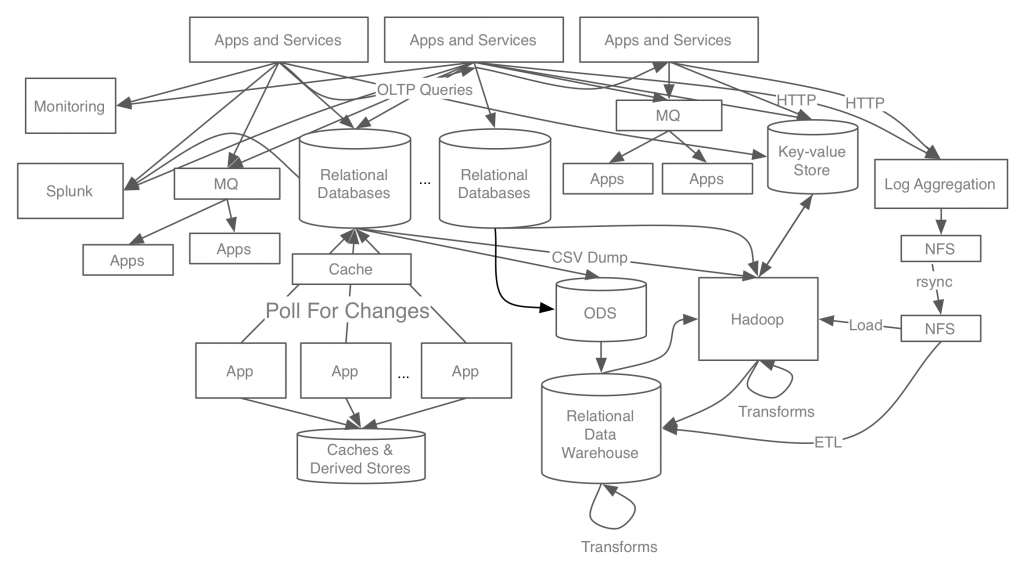
\includegraphics[width=\linewidth]{images/linkedin-data-flow-ugly.png}
	\caption{The tangled data systems at LinkedIn in the old day \cite{eventstreamingplatform}.}
	\label{fig:tangledsystem}
\end{figure}

This problem can be tackled by using stream processing in event-driven systems. In such systems, every operation, state change or any information can be recorded in form of an event. Events from all services are gathered and written orderly to an append-only log called event stream. On the contrary to the previous approach where data is encapsulated in each service, this stream is used as the single source of truth shared by all services. Any data service in the system can consume and process this log of raw events using stream processing to generate a local replication of the current system state. This log-centric design fits seamlessly into a distributed environment with numerous moving components to allow data to be replicated among services with minimal coupling \cite{logjaykreps}. Moreover, services also have the flexibility to derive different data structures from the raw events to match their specific access pattern. The task of data representation is now done at individual data service instead of in the central data store. This is referred by Martin Kleppmann as turning the database inside out \cite{kleppmann2016making}. The result is a more neatly organized system with every services synchronize and communicate via the event streams.

\begin{figure}[h]
	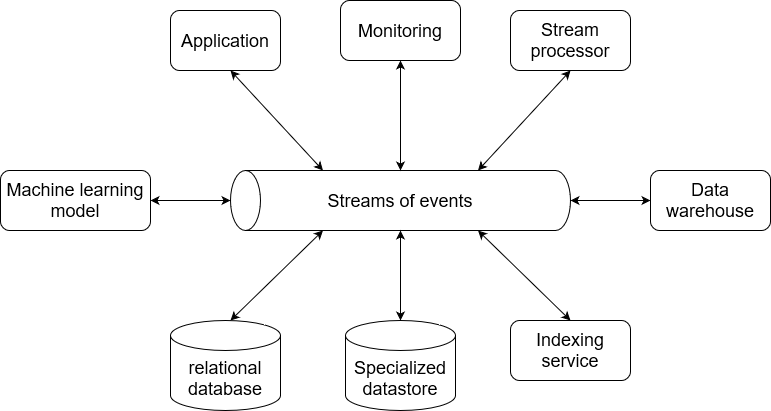
\includegraphics[width=\linewidth,height=7cm]{images/eventstreamprocessing.png}
	\caption{System with streams of events as the single source of truth.}
	\label{fig:eventstreamprocessingsystem}
\end{figure}

\section{\acrlong{esp} Platform}
An \acrlong{esp} platform must facilitate the construction of software systems revolving around streams of events. Therefore, it must have a number of fundamental capabilities. Firstly, it must provide the mechanism for events storage. Optimally, it should also support the option to persist events for an infinite period of time since this will be the single source of truth that the entire system depends on. Accessing interface must be provided for applications to publish and consume events. The platform should also enable the processing on the events streams either by providing a native stream processing tool or integrating with external stream processing framework. Moreover, the platform should come with ready-to-be-used tools to integrate with a wide range of existing data systems effortlessly including also legacy systems.

The order of events must be preserved by the platform throughout their entire life cycle: in storage, transit and under process. All of these capabilities should be in a real-time, high throughput, scalable and highly reliable fashion so that the platform would not become the bottleneck in the system. Finally, the platform must have a rich set of utility tools for monitoring and management.



